\onecolumngrid
\section*{End Matter}
\twocolumngrid

\begin{table*}[]
\caption{Summary of the surrogate models constructed in this work. For each model, we list its length, maximum initial eccentricity ($e_{\rm max}$), number of training points ($N_{\rm train}$), and starting frequency range ($f_0$) for a $10M_\odot$ binary. All the eccentric surrogates are built for mass ratios $\in [1,6]$, while the (time-parameterized) quasi-circular surrogate (last row) is built for mass ratios $\in [1,8]$. We compare the number of basis functions required for the eccentric residuals ($\Delta A, \Delta \phi$) and the median/maximum mismatch against the base model \inspiralesigma{} for both time ($t$) and mean anomaly ($l$) parameterizations.}
\label{tab: surrogate-metrics}
\setlength{\tabcolsep}{5pt}
\begin{tabular*}{\textwidth}{@{\extracolsep{\fill}} c c c c c c c c}
\toprule
\multicolumn{1}{c}{Length} & \multicolumn{1}{c}{$e_{\rm max}$} & \multicolumn{1}{c}{$N_{\rm train}$} & \multicolumn{1}{c}{$f_0$ @ $10 M_\odot$} & \multicolumn{2}{c}{\# Basis functions $(\Delta A, \Delta \phi)$} & \multicolumn{2}{c}{Mismatch @ $10 M_\odot$ (median, max)} \\
\cmidrule(lr){5-6} \cmidrule(lr){7-8}
($10^3 M$) & & & (Hz) & $t$-param. & $l$-param. & $t$-param. & $l$-param. \\
\midrule
23   & 0.067 & 504  & 57--73 & 57, 49   & 10, 6   & $4.9 \times 10^{-6}, 1.0 \times 10^{-2}$ & $2.6 \times 10^{-8}, 9.0 \times 10^{-5}$ \\
105  & 0.11 & 672  & 32--42 & 167, 143 & 12, 8   & $2.4 \times 10^{-4}, 2.6 \times 10^{-1}$ & $6.7 \times 10^{-8}, 3.5 \times 10^{-5}$ \\
510  & 0.21 & 864  & 17--24 & 430, 363 & 15, 11  & ---                            & $1.4 \times 10^{-7}, 1.2 \times 10^{-5}$ \\
1250 & 0.36 & 1152 & 10--17 & 635, 589 & 31, 16  & ---                            & $1.2 \times 10^{-6}, 7.6 \times 10^{-5}$ \\
2770 & 0.43 & 1404 & 7.2--12 & 884, 795 & 36, 21  & ---                            & $3.2 \times 10^{-6}, 5.3 \times 10^{-5}$ \\
\midrule
\multicolumn{8}{c}{Quasi-circular model}\\
\midrule
6020 & 0 & 50 & 7.2--10 & \multicolumn{2}{c}{4, 4 $(A_{22}, \phi_{22})$} & \multicolumn{2}{c}{$1.9 \times 10^{-9}, 3.1 \times 10^{-8}$} \\
\bottomrule
\end{tabular*}
\end{table*}

\textit{Appendix A: Mean anomaly domain surrogate construction steps---}
Collectively denoting the eccentric residuals $\{\Delta A$, $\Delta \phi$, $\phi_{\rm{res}}\}$ by $\bm{f}$, we list the steps of constructing the mean anomaly parameterized surrogate below. 
\begin{enumerate}
    \item Assuming a training set of $N_{\rm{train}}$ inspiral-only waveforms with parameters $\{\param_i\}_{i=1}^{N_{\rm{train}}}$, we extract the \textit{unwrapped} mean anomaly evolution as a function of time $l(t; \param_i)$ from the waveform model's orbital dynamics solver.
    \item We find the mean-anomaly extent of each waveform $\Delta l(\param_i) = l(t=0; \param_i) - l(t=t_0; \param_i)$, where $t_0$ is the starting time of the particular waveform. We then calculate the maximum possible common mean anomaly extent $L$ of the training space waveforms by calculating the minimum of their extents, i.e. $L = \mathrm{min}_i\, \Delta l(\param_i)$. We also denote by $T_L(\param_i)$ the time durations of the waveforms having a mean anomaly extent of $L$. 
    \item We define the \textit{shifted mean anomaly}, 
    \begin{equation}
        l_s(t; \param) = l(t; \param) - l(t=0; \param),
        \label{eqn: shifted mean anomaly}
    \end{equation}
    and model all the eccentric residuals ($\bm{f}$) against it, i.e. as $\bm{f}(l_s; \param_i)$ in $l_s \in [-L, 0]$. We make surrogates $\bm{f_s}(l_s; \param)$ for these data-pieces.
    We set $\phi_{22}(l_s=-L; \param)=\phi_{22}(l_s=-L; \eref=\lref=0, \bm{\theta'})=0$, thus ensuring that $\Delta \phi_1(l_s=-L; \param)=0$ (c.f. Eq. \ref{eqn: residual-phase}).
    \item We also construct a surrogate $l_s^{\rm{sur}}(t; \param)$ of the shifted mean anomaly as a function of time for $t \in [-T_{\rm{min}}^L, 0]$, where $T_{\rm{min}}^L = \mathrm{min}_i \, T_L(\param_i)$ is the maximum possible surrogate length in time for a training space with mean-anomaly extent $L$. Since $l_s$ is a monotonically increasing, non-oscillatory function of time (see Fig. \ref{fig: chirp}), its surrogate requires only a few $(<10)$ basis functions.
    \item Using the shifted mean anomaly surrogate, we can get the surrogates of the eccentric data-pieces as a function of time: $\bm{f_s}(t; \param) = \bm{f_s}(l_s=l_s^{\rm{sur}}(t; \param); \param)$, where $t \in [-T_{\rm{min}}^L, 0]$.
    \item For \textit{both} time-parameterized and mean anomaly-parameterized surrogates, variations in the eccentric residuals $\Delta A$ and $\Delta \phi$ across the parameter space at a particular EI node are significantly simplified when parameterized by the instantaneous values of eccentricity ($e_{\rm{EI}}^k$) and mean anomaly ($l_{\rm{EI}}^k$) at the EI nodes (labeled by the index $k$), instead of their values $(e_{\rm{ref}}, l_{\rm{ref}})$ at a fixed reference time $t_{\rm{ref}}$. This is illustrated in Fig. \ref{fig: parameter-space-variation} for mean anomaly parameterized $\Delta A$ at a shifted mean anomaly EI node. However, in the mean anomaly parameterized case, we find that the parameter space variations in $\phi_{\rm{res}}$ at the shifted mean anomaly EI nodes show oscillations. We found that fixing the eccentric residual phase and the monotonic trend initially to zero, i.e. $\Delta \phi(l_s=-L)=\phi_{\rm{res}}(l_s=-L)=0$ simplifies their structure. This choice still respects the zero starting $(2,2)$-mode phase condition $\Delta \phi_1(l_s=-L; \param)=0$. Hence, we use these initially zeroed-out $\Delta \phi$ and $\phi_{\rm{res}}$ for the mean anomaly parameterized surrogate.
    \item Lastly, we build surrogates of the eccentricity $e(l_s; \param)$ and the (unwrapped) mean anomaly $l(l_s; \param)$ evolution as a function of $l_s$, to evaluate the values of eccentricity ($e_{\rm{EI}}^k$) and (wrapped) mean anomaly ($l_{\rm{EI}}^k$) at the shifted mean anomaly EI nodes $l_s=L_s^k$ at any $\param$ \footnote{Similarly, we build surrogates of the eccentricity $e(t; \param)$ and the (unwrapped) mean anomaly $l(t; \param)$ evolution as a function of $t$ for the time-parameterized surrogates constructed in this work.}. However, since $l_s(t; \param) = l(t; \param) - l(t=0; \param)$, we simply build a parameter space fit for $l(t=0; \param)$ to get the mean anomaly at EI nodes as $l(l_s=L_s^k; \param) = L_s^k + l(t=0; \param)$. 
\end{enumerate}

\begin{figure}
    \centering
    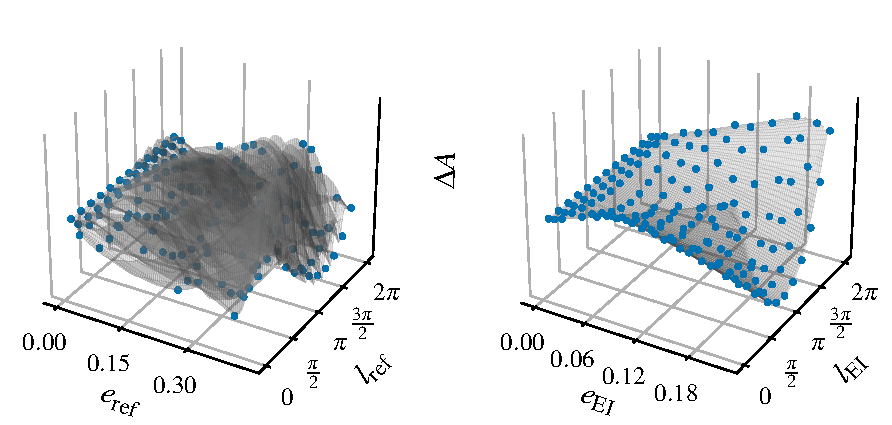
\includegraphics[width=\columnwidth, trim=0.35cm 0.125cm 0.2cm 0.8cm, clip ]{Figures/param-space-variation.pdf}
    \caption{Variation of the eccentric residual amplitude $\Delta A$ at a single empirical interpolation (EI) node across the parameter space for a fixed mass ratio $(q = 3.2)$ for the $2.77 \times 10^6M$ long surrogate. The parameterization in terms of instantaneous values of eccentricity ($e_{\rm{EI}}$) and mean anomaly ($l_{\rm{EI}}$) at the EI nodes (right) yields smoother variation than a parameterization in terms of their values $e_{\rm{ref}}$ and $l_{\rm{ref}}$ at a fixed reference time $t_{\rm{ref}}$ (left). The simplified structure allows for the construction of accurate parametric fits with relatively fewer training space points. $\Delta A$ at a shifted mean anomaly EI node is shown here, and a similar simplification is obtained at time EI nodes as well. 
    }
    \label{fig: parameter-space-variation}
\end{figure}

\begin{figure*}
    \centering
    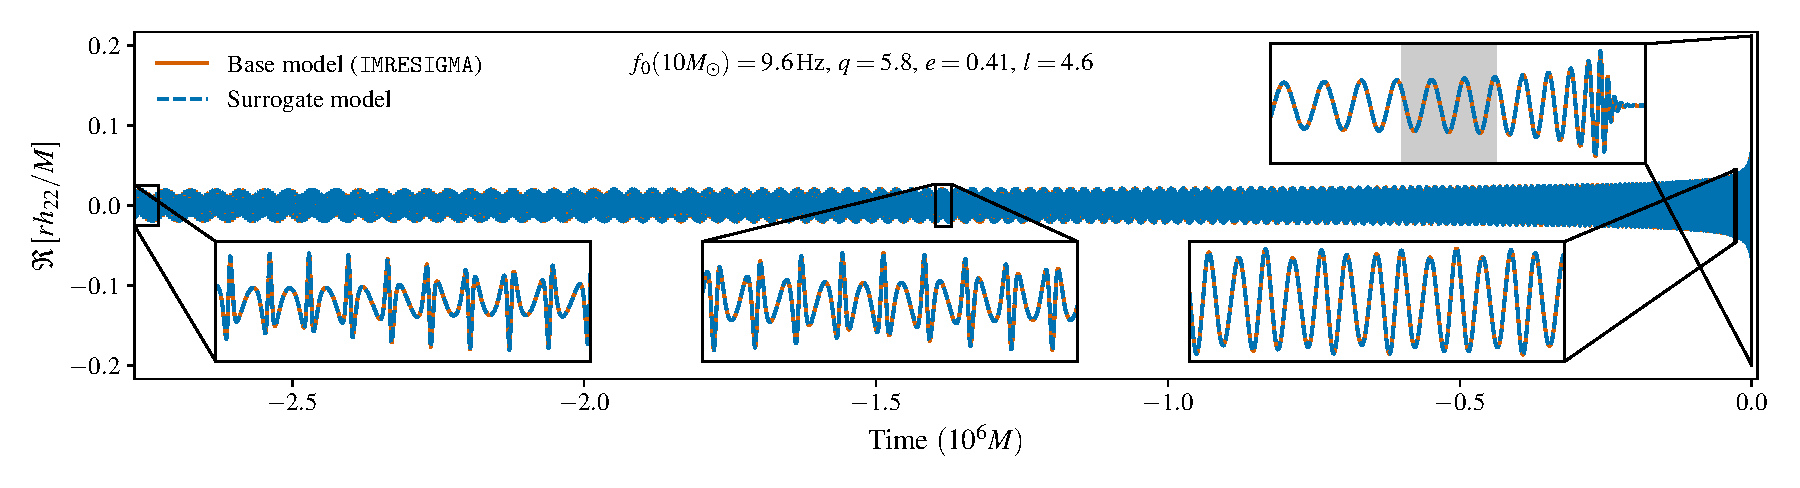
\includegraphics[width=\textwidth, trim=0.54cm 0.53cm 0.53cm 0.52cm, clip]{Figures/IMR-sur-comparison.pdf}
    \caption{The $2.77 \times 10^6M$ long surrogate waveform for \inspiralesigma{} smoothly attached to the plunge-merger-ringdown piece coming from the quasi-circular numerical relativity surrogate \nrsur{} \citep{Varma:2019csw} to produce a hybridized IMR surrogate waveform (blue), and its comparison against \imresigma{} (orange) that employs the same attachment on \inspiralesigma{} \citep{Paul:2024ujx, esigmapy}. The parameters at the start of the waveform are also listed and correspond to the case yielding the worst mismatch ($5.3 \times 10^{-5}$) between the surrogate and \inspiralesigma{} at $10M_\odot$. The surrogate waveform is time and phase shifted by their optimal values found during the match computation.
    The top inset also shows the window (gray band) in which the surrogate is smoothly attached to the plunge-merger-ringdown piece. As highlighted via the insets, the hybridized surrogate waveform remains faithful to the base \imresigma{} waveform from early inspiral through merger-ringdown.} 
    \label{fig: IMR-surrogate}
\end{figure*}

\textit{Appendix B: Summary of all surrogate models---}
To highlight the enhanced scaling and accuracy of the mean anomaly parameterization, we build eccentric, non-spinning surrogates of increasing time durations for the waveform model \inspiralesigma{} using both time and mean anomaly parameterizations. Their metrics are summarized in Table \ref{tab: surrogate-metrics}. 
All the eccentric surrogates cover mass ratios $m_1/m_2\in[1, 6]$, with the maximum starting eccentricity $(e_{\rm{max}})$ chosen such that the eccentricity decays down sufficiently by the end of the inspiral ($e(t=0) \lesssim 0.005$). As required within the \esigmahm{} framework~\citep{Paul:2024ujx, esigmapy}, this allows smooth attachment of a quasi-circular plunge-merger-ringdown piece to construct a hybrid  IMR waveform, as shown in Figure \ref{fig: IMR-surrogate}. Table \ref{tab: surrogate-metrics} also lists the range of minimum starting frequency $f_0$ a $10M_\odot$ binary can be started from and the number of basis functions required to represent the training space of eccentric residuals $\Delta A$ and $\Delta \phi$ within an error threshold of $10^{-5}$ (c.f. Figure \ref{fig: surrogate-scaling}). Only a few basis functions ($\lesssim 10$) are required for the other surrogate data-pieces $\phi_{\rm{res}}(t), \phi_{\rm{res}}(l_s), l_s(t), e(t), e(l_s)$ and $l(t)$ due to their non-oscillatory nature, and are similar in number for both the time and the mean anomaly parameterized approaches and hence are not listed. The median and worst mismatches, computed using the zero-detuning high-power noise power spectral density for the advanced LIGO detector~\citep{LIGO-T0900288-v3, LIGO-T070247-v1} for the full surrogate lengths for a $10M_\odot$ binary against $10,000$ \inspiralesigma{} waveforms randomly sampled across the parameter space of the surrogates, are also listed. We do not proceed beyond basis construction for time-parameterized surrogates longer than $105 \times 10^3M$ because of the large number of basis functions involved, and hence do not have their mismatch data. Lastly, the metrics for the time-parameterized quasi-circular surrogate built for mass ratios $m_1/m_2\in [1,8]$ are also listed, including the number of basis functions required for the quasi-circular amplitude $A_{22}$ and phase $\phi_{22}$. 
The basis construction error thresholds for non-oscillatory data pieces, namely the quasi-circular $A_{22}(t)$ and $\phi_{22}(t)$, and $\phi_{\rm{res}}(t), \phi_{\rm{res}}(l_s), l_s(t), e(t), e(l_s)$ and $l(t)$, are chosen to retain the maximum number of basis functions without noise, as determined through visual inspection.

All the time-domain data pieces are sampled at a uniform spacing of $10M$, except the quasi-circular data pieces at $\simeq 5M$, while the mean anomaly-domain data pieces are sampled uniformly at $2 \pi/100$ (i.e., 100 points per radial orbit). We use linear interpolation over these time/mean anomaly grids to evaluate the surrogates over any user-desired time grid.




